%%%%%%%% this is the Preliminary results

%\documentclass[12pt, amstex, letterpaper] {report} %{article}


\usepackage[margin=1in]{geometry}
\topmargin -0.5in \textwidth 6.5in \textheight 9in
\footskip .5in
\headheight 0.3in


\usepackage{Sweave}

\DefineVerbatimEnvironment{Sinput}{Verbatim} {xleftmargin=0em,frame=single}
\DefineVerbatimEnvironment{Soutput}{Verbatim} {xleftmargin=0em,frame=single}

\usepackage{amssymb, mathrsfs, amsmath, amsfonts}
\usepackage{enumerate, comment}
\usepackage{hyperref, natbib,apalike, float} %cite
\usepackage{color, multirow, setspace, fancyhdr,graphicx}
\usepackage{undertilde}
\usepackage[bottom]{footmisc}
\usepackage{graphicx}
\usepackage{framed}
\usepackage{subcaption}
\usepackage{amsthm}

%\doublespacing
\pagestyle{empty}
\pagestyle{fancy}
\lhead{ }
%\rhead{May 2016}
\fancyfoot{ }
\rfoot{Dissertation $|$ \thepage}
\lfoot{Chris Vanlangenberg}
\date{}

\includecomment{comment}

\newtheorem{theorem}{Theorem}[section]
\newtheorem{defn}{Definition}[section]
\newtheorem{prop}{Proposition}
\newcommand{\pro}[1]{\begin{prop}{#1}\end{prop}}

%\newtheorem{proof}{proof}
\newtheorem{rmk}{Remark}
\newcommand{\rmark}[1]{\begin{rmk}{#1}\end{rmk}}

\numberwithin{equation}{section}
\renewcommand{\footrulewidth}{0.1pt}
\renewcommand{\headrulewidth}{0.1pt}


\newcommand{\eqn}[1]{\begin{equation}{#1}\end{equation}}

\newcommand{\beq}{\begin{equation}}
\newcommand{\eeq}{\end{equation}}
%\renewcommand\refname{Literature}
\newcommand{\blue}[1]{\textcolor{blue}{\emph{#1}}}
\newcommand{\red}[1]{\textcolor{red}{\emph{#1}}}
\newcommand{\twoc}[2]{{\textcolor{blue}{#1}} and {\textcolor{red}{#2}}}


\newcommand{\xn}{x_1,\ldots, x_n}
\newcommand{\Xn}{X_1,\ldots, X_n}
\newcommand\floor[1]{\lfloor{#1}\rfloor}
\newcommand\ceil[1]{\lceil{#1}\rceil}

\newcommand{\X}{\mathcal{X}}
\newcommand{\Sp}{\mathbb{S}}
\newcommand{\R}{\mathbb{R}}
\newcommand{\C}{\mathbb{C}}
\newcommand{\pd}{positive definite }



\newcommand{\code}[1]{{\small\texttt{#1}}}
\newcommand{\pkg}[1]{{\normalfont\textsf{#1}}}
\newcommand{\var}[1] {{\normalfont\textbf{#1}}}
\newcommand{\Cm}{$C_m(\phi_P, \phi_Q)\ $}

\newcommand{\jun}{\cite{JunStein2008}}
%\begin{document}
%\section{Methods}

%\subsection{For data generation part:}

%%%%%%%%%%%%%%%%%%%%%%%%%%%%%%%%%%
%\subsubsection{Model comparison}
%%%%%%%%%%%%%%%%%%%%%%%%%%%%%%%%%%

{\bf Simulated data sample:}

\begin{figure}[H]
\label{grid_plot_model2}
\begin{center}
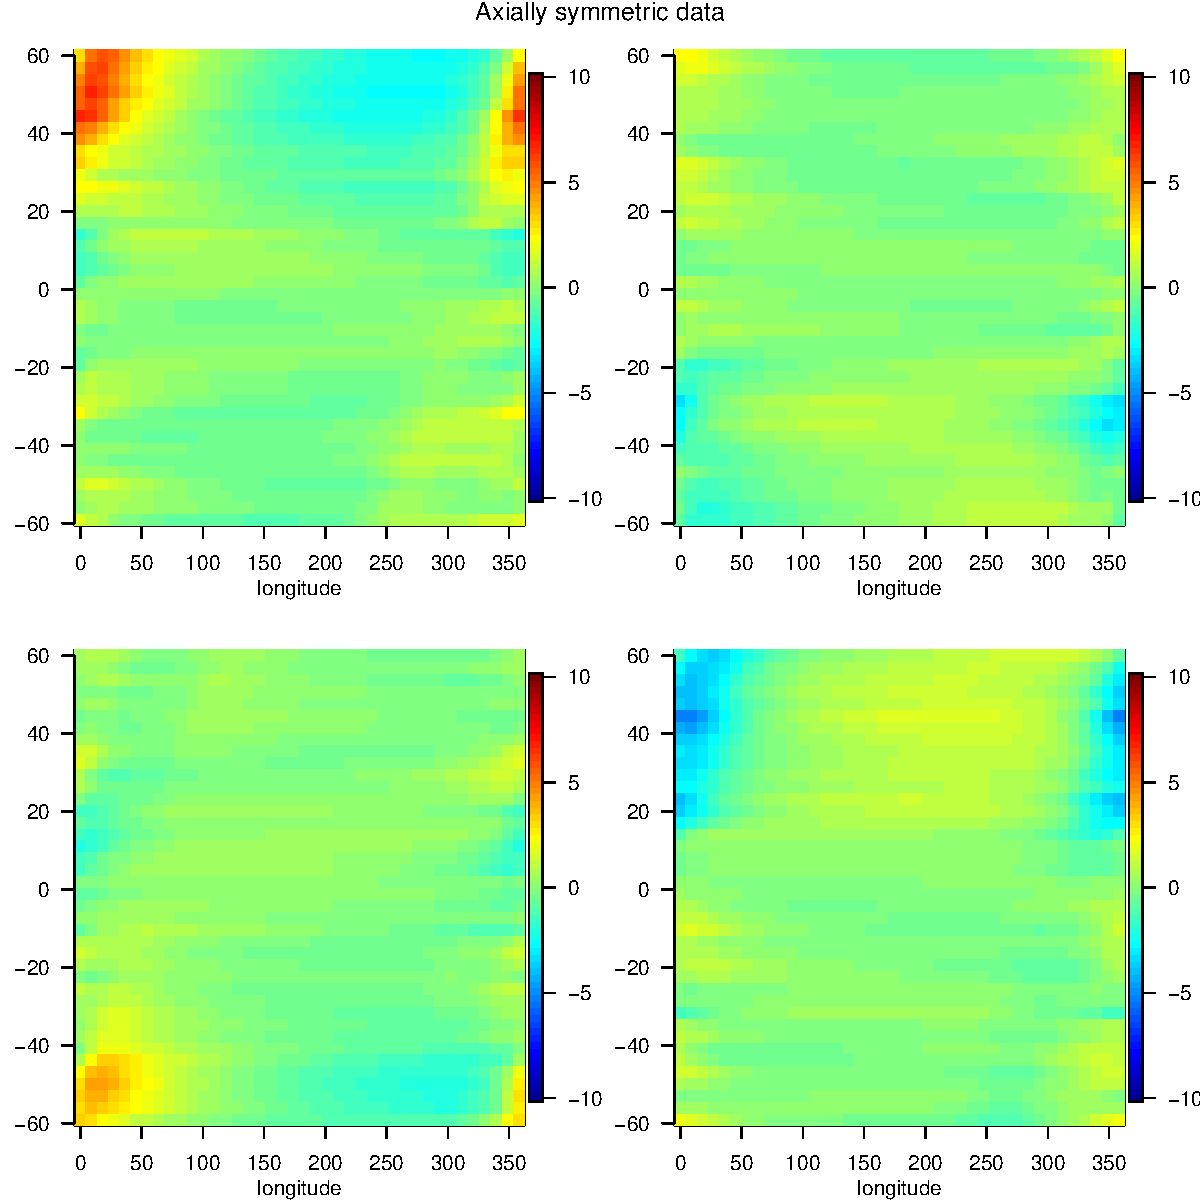
\includegraphics [scale=1]{graphs/Data_sample_120_model2.pdf}
\caption{Four consecutive axially symmetric data snapshots based on model 2, grid resolution $2^0\times 1^0$ (data scale -10 and 10).}
\end{center}
\end{figure}

\newpage
{\bf Comprison of the proposed models with MOM estimates:}

\begin{itemize}
\item Model 1\\

\begin{figure}[H]
\begin{center}
\fbox{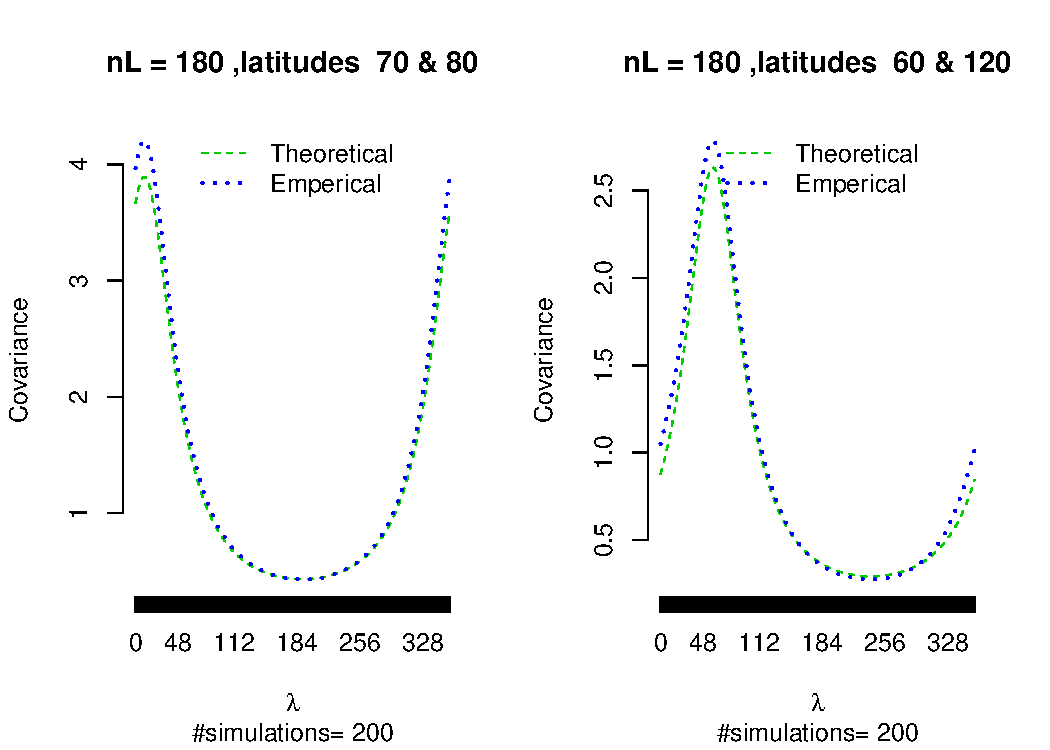
\includegraphics [width=12cm,height=12cm,keepaspectratio]{graphs/Model1.pdf}}
\caption{Cross covariance comparison of model1}
\end{center}
\end{figure}

\newpage
\item Model 2
\begin{figure}[H]
\begin{center}
\fbox{\includegraphics [width=12cm,height=12cm,keepaspectratio]{graphs/Model2.pdf}}
%\includegraphics [width=6in, height=3in]{Model2.pdf}
\caption{Cross covariance comparison of model2}
\end{center}
\end{figure}


\item Model 3
\begin{figure}[H]
\begin{center}
%\includegraphics [scale=.6]{Model3.pdf}
\fbox{\includegraphics [width=12cm,height=12cm,keepaspectratio]{graphs/Model3.pdf}}
\caption{Cross covariance comparison of model3}
\end{center}
\end{figure}

\end{itemize}


%\end{document}